%%%%%%%%%%%%%%%%%%%%%%%%%%%%%%%%%%%%%%%%%%%%%%%%%%%%%%%%%%%%%%%%%%%%%%%
% 1. Document class
%%%%%%%%%%%%%%%%%%%%%%%%%%%%%%%%%%%%%%%%%%%%%%%%%%%%%%%%%%%%%%%%%%%%%%%

\documentclass[conference]{IEEEtran}

%%%%%%%%%%%%%%%%%%%%%%%%%%%%%%%%%%%%%%%%%%%%%%%%%%%%%%%%%%%%%%%%%%%%%%%
% 2. Packages
%%%%%%%%%%%%%%%%%%%%%%%%%%%%%%%%%%%%%%%%%%%%%%%%%%%%%%%%%%%%%%%%%%%%%%%

% \IEEEoverridecommandlockouts
% The preceding line is only needed to identify funding in the first footnote. If that is unneeded, please comment it out.
\usepackage{cite}
\usepackage{amsmath,amssymb,amsfonts}
\usepackage{algorithmic}
\usepackage{graphicx}
\usepackage{textcomp}
\usepackage{xcolor}
\def\BibTeX{{\rm B\kern-.05em{\sc i\kern-.025em b}\kern-.08em
    T\kern-.1667em\lower.7ex\hbox{E}\kern-.125emX}}

%%%%%%%%%%%%%%%%%%%%%%%%%%%%%%%%%%%%%%%%%%%%%%%%%%%%%%%%%%%%%%%%%%%%%%%
% 3. Title
%%%%%%%%%%%%%%%%%%%%%%%%%%%%%%%%%%%%%%%%%%%%%%%%%%%%%%%%%%%%%%%%%%%%%%%

\begin{document}

\title{Reto II: Interpolación y Ajuste de Curvas \\
    \vspace{-1ex}
    {\footnotesize Desplazamiento de una hormiga en una Superficie}
}

\author{
    \IEEEauthorblockN{Alejandro Morales Contreras}
    \IEEEauthorblockA{
    \textit{Pontificia Universidad Javeriana}\\
    Bogotá, Colombia \\
    a.moralesc@javeriana.edu.co
    }
\and
    \IEEEauthorblockN{Carlos Miguel Sánchez Loreto}
    \IEEEauthorblockA{
    \textit{Pontificia Universidad Javeriana}\\
    Bogotá, Colombia \\
    sa-carlos@javeriana.edu.co}
\and
    \IEEEauthorblockN{Santiago Vásquez Sánchez}
    \IEEEauthorblockA{
    \textit{Pontificia Universidad Javeriana}\\
    Bogotá, Colombia \\
    santiago.vasquezs@javeriana.edu.co}
}

\maketitle

% Cambiar el título de Abstract a Resumen

\renewcommand{\abstractname}{Resumen}
\makeatletter
  \ifCLASSOPTIONconference
\def\abstract{\@IEEEtweakunitybaselinestretch{1.15}\bfseries
    \if@twocolumn
      \@IEEEabskeysecsize\noindent\textit{\abstractname}---\relax
    \else
      \bgroup\par\addvspace{0.5\baselineskip}\centering\vspace{-1.78ex}\@IEEEabskeysecsize\textbf{\abstractname}\par\addvspace{0.5\baselineskip}\egroup\quotation\@IEEEabskeysecsize%
    \fi\@IEEEgobbleleadPARNLSP}
\makeatother

%%%%%%%%%%%%%%%%%%%%%%%%%%%%%%%%%%%%%%%%%%%%%%%%%%%%%%%%%%%%%%%%%%%%%%%
% 4. Body
%%%%%%%%%%%%%%%%%%%%%%%%%%%%%%%%%%%%%%%%%%%%%%%%%%%%%%%%%%%%%%%%%%%%%%%

\begin{abstract}
Este documento busca informar, explicar, comparar y graficar la reconstrucción de una figura, cuya trayectoria está representada por una serie de parejas ordenadas $(x,y$). Se implementan diferentes métodos de interpolación y ajuste de curvas con el fin de encontrar una buena aproximación de la trayectoria deseada, así mismo, se define cual de los métodos utilizados es el más apropiado para la resolución de problemas de reconstrución de figuras con el menor error posible.
\end{abstract}

%%%%%%%%%%%%%%%%%%%%%%%%%%%%%%%%%%%%%%%%%%%%%%%%%%%%%%%%%%%%%%%%%%%%%%%
% 4.1. Introducción
%%%%%%%%%%%%%%%%%%%%%%%%%%%%%%%%%%%%%%%%%%%%%%%%%%%%%%%%%%%%%%%%%%%%%%%

\section{Introducción}

A continuación se pretende mostrar el análisis, implementación y resultados obtenidos del reto II de la materia, sobre el ajuste de curvas mediante interpolación. Se abordan los conceptos de interpolación cúbica mediante Splines e interpolación de Lagrange, con el fin de encontrar una solución al problema planteado. La implementación de los métodos fue llevada a cabo en el lenguaje de programación R, mediante la herramienta RStudio. Así mismo, se utilizaron otras herramientas como Wolfram Alpha para apoyar los procedimientos implementados. \par

Inicialmente, se hará un análisis del marco teórico sobre los conceptos que se van a tratar. Después, se mostrará el problema planteado. Finalmente, se procederá a exponer la solución implementada, así como los resultados obtenidos. \par

%%%%%%%%%%%%%%%%%%%%%%%%%%%%%%%%%%%%%%%%%%%%%%%%%%%%%%%%%%%%%%%%%%%%%%%
% 4.2. Marco Teórico
%%%%%%%%%%%%%%%%%%%%%%%%%%%%%%%%%%%%%%%%%%%%%%%%%%%%%%%%%%%%%%%%%%%%%%%

\section{Marco Teórico}

\subsection{Interpolación}

En el subcampo de las matemáticas del análisis numérico, la obtención de nuevos puntos en relación al conocimiento de un conjunto de puntos se denomina interpolación. El problema general de la interpolación se presenta cuando se conoce únicamente una serie de puntos, de la cual se busca extraer información \par

\[ (x_0, y_0), (x_1, y_1), ..., (x_n, y_n) \] \par

y se busca aproximar una función que pase por todos los puntos. \par

La idea de la interpolación es poder estimar $f(x)$ para un valor de $x$ arbitrario, a partir de la construcción de una curva o superficie que une los puntos donde se han realizado las mediciones y cuyo valor si se conoce. Se asume que el punto arbitrario $x$ se encuentra dentro de los límites de los puntos de medición, es decir, de los valores extremos $(x_0, y_0)$ y $(x_n, y_n)$. En caso de que el punto a estimar se encuentre por fuera de este rango, se estaría hablando de extrapoliación. \cite{b2}\par

\subsection{Interpolación de Lagrange}

Cuando se desea obtener el polinomio de interpolación en forma normal el costo aritmético del sistema de ecuaciones lineales del cual se requiere la resolución es del orden $n^3$, siendo $n$ el número de nodos. \par

Para reducir este costo, se puede tomar una base del espacio formada por polinomios $Lin(x),i=0, \ldots, n$, dependientes de las abscisas $x_0, x_1, \ldots, x_n$, de los nodos considerados, siendo este el caso de los polinomios de L'Lagrange. Estos polinomios logran determinar una expresión explícita del polinimio de interpolación. \par

\subsubsection{Existencia del polinomio de interpolación}

Sea $Lin(x)$ un polinomio de grado $n$, que se anule en todos los puntos $x_j, j = 0, 1, ..., n$, salvo en el i-ésimo, donde vale $1$; es decir, tal que

\[ Li(x_j) = 0 \text{ si } j!= i \text{ y } Li(x_i) = 1 \]\

La existencia de este polinomio se deriva del resultado anterior, pero puede obtenerse directamente, sin necesidad de resolver un sistema, gracias a la siguiente fórmula de Lagrange \cite{b1}\par

\[ \frac{(x-x_0)\ldots(x-x_{i-1})(x-x_{i+1})\ldots(x-x_n)}{(x_1-x_0)\ldots(x_i-x_{i-1})(x_i-x_{i+1})\ldots(x_i-x_n)} \]

Es inmediato comprobar entonces que el polinomio 
\[ P_n(x) = y_0 L_0(x) + y_1 L_1(x) + y_2 L_2(x) + ... + y_n L_n(x) \]

Donde, \par

\[ P_n(x_i) = y_i, i = 0,1,2,...,n \]\

La unicidad se puede verificar basandose en el hecho de que un polinomio de grado n puede tener como maximo n raíces. Si dos polinomios de grado menor o igual a grado n interpolan n+1 puntos, su diferencia se anula en dichos puntos, por lo que bajo la teorica matematica, sólo puede ser el polinomio idénticamente nulo. \cite{b1}\par

\subsection{Interpolación mediante Splines}

La interpolación de Splines es usada normalmente para el diseño por computada. La idea central de esta interpolacion es que en vez de usar solo un polinomio para interpolar todos los datos, podemos segmentar polinomios y unirlos adecuadamente para formal la interpolación. \par

De esta forma, se puede entender que una función spline está formada por varios polinomios, cada uno unido bajo ciertas condiciones de continuidad y con un intervalo definido para cada uno de estos.\par

\subsubsection{Implementación Matemática}

Dada un conjunto de datos $[(x_0,x_0),...,(x_n,y_n)]$. Dado $k$ un número entero positivo, una función de interpolación splines de grado $k$, para la tabla de datos, es una función $s(x)$ tal que:\cite{b2}\par

\begin{itemize}
    \item $s(x_i) = y_i$, para toda $i$.
    \item $s(x)$ es un polinomo de grado $\leq k$ en cada subintervalo $[x_{i-1},x_i]$.
    \item $s(x)$ tiene derivada continua hasta de orden $k-1$ en $[x_0,x_n]$.
\end{itemize}

%
%%%%%%%%%%%%%%%%%%%%%%%%%%%%%%%%%%%%%%%%%%%%%%%%%%%%%%%%%%%%%%%%%%%%%%
% 4.3. Problema Planteado
%%%%%%%%%%%%%%%%%%%%%%%%%%%%%%%%%%%%%%%%%%%%%%%%%%%%%%%%%%%%%%%%%%%%%%%

\section{Problema Planteado}

El problema planteado, consiste en la reconstrucción de la trayectoria que toma el desplazamiento de una hormiga, de acuerdo a la información dada. Esta información es presentada como 64 puntos $(x,y)$, que fueron tomados cada 2 segundos. A continuación se presenta ambos conjuntos de pares. \par

$x=($6.7, 6.0, 5.0, 4.3, 3.5, 2.8, 2.3, 1.7, 1.8, 2.5, 3.0, 3.6, 4.2, 4.5, 5.2, 5.6, 5.3, 5.2, 5.1, 4.9, 4.7, 4.8, 5.2, 5.6, 6.0, 6.3, 7.2, 7.3, 7.4, 7.3, 7.8, 8.4, 8.8, 8.9, 9.0, 9.1, 9.2, 9.6, 10.1, 10.8, 11.5, 11.7, 11.4, 10.7, 11.4, 11.8, 12.6, 13.0, 13.6, 13.9, 14.0, 13.7, 13.2, 12.9, 12.8, 12.7, 12.5, 12.2, 12.1, 12.0, 11.9, 11.8, 11.6, 11.5$)$ \par

$y=($3.0, 3.6, 4.9, 6.3, 8.0, 8.6, 9.7, 10.7, 11.3, 11.5, 11.2, 10.7, 10.0, 9.6, 8.6, 9.6, 11.0, 12.2, 13.3, 14.0, 15.2, 16.2, 16.6, 16.5, 15.5, 14.0, 11.7, 13.8, 14.7, 16.0, 17.4, 17.6, 17.3, 16.3, 15.4, 14.0, 12.3, 14.5, 16.1, 16.9, 16.5, 15.7, 14.4, 11.2, 12.0, 12.4, 13.5, 14.2, 14.4, 14.1, 13.7, 13.0, 12.2, 11.6, 11.2, 10.9, 10.5, 9.5, 8.3, 7.6, 6.7, 6.0, 5.0, 4.5$)$ \par


\vspace{-1em}

\begin{figure}[ht!]
\centering
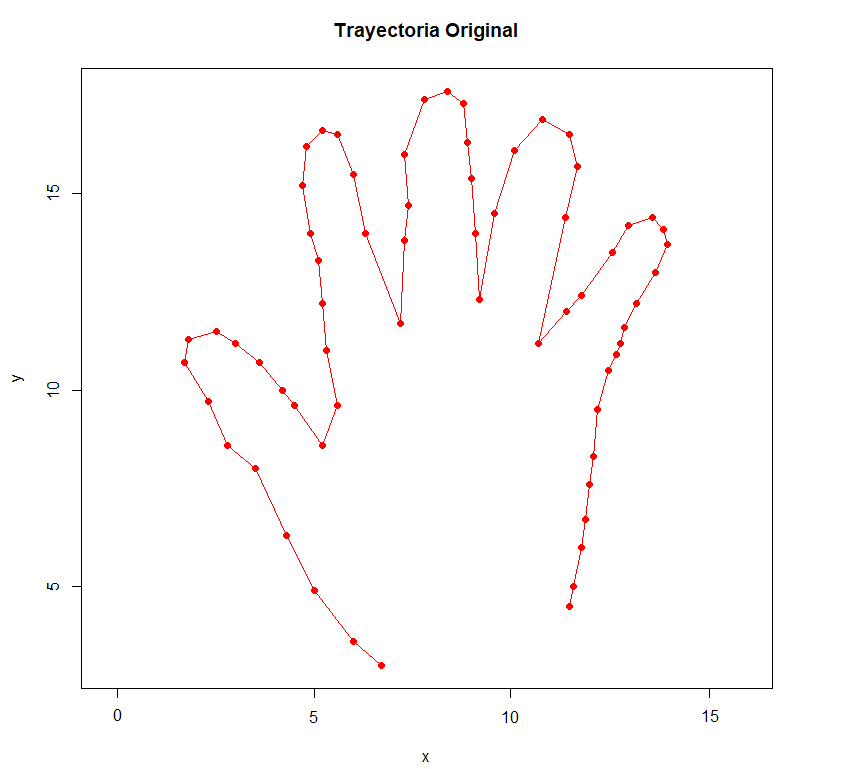
\includegraphics[scale=0.33]{img/TrayectoriaOriginal.PNG}
\vspace{-1em}
\caption{Trayectoria no interpolada de la hormiga}
\label{fig:trayectoria-original}
\end{figure} 

Adicionalmente, se busca también la optimización de la solución que se obtenga. Es decir, se espera también reducir la cantidad de puntos hasta la mínima cantidad posible, manteniendo al mínimo el error.\par

%%%%%%%%%%%%%%%%%%%%%%%%%%%%%%%%%%%%%%%%%%%%%%%%%%%%%%%%%%%%%%%%%%%%%%%
% 4.4. Solución
%%%%%%%%%%%%%%%%%%%%%%%%%%%%%%%%%%%%%%%%%%%%%%%%%%%%%%%%%%%%%%%%%%%%%%%

\section{Solución}

El problema fue resuelto en el lenguaje de programación R, mediante el uso de librerías en conjunto con implementaciones propias. El código fuente puede ser encontrado en el siguiente repositorio: \par

https://github.com/AlejandroMoralesContreras/analisis-numerico.git \par

\subsection{Librerías Utilizadas en R}

\subsubsection{Librería stats}

Esta librería fue utilizada para la implementación del método de interpolación mediante Splines. Se utilizó la función $splinefun(x, y)$, la cual retorna la función interpolante dado el conjunto de puntos $(x,y)$.

\subsection{Reconstrucción mediante Lagrange}

La primera solución que se planteó fue utilizar una función interpolatoria de Lagrange implementada en clases, que toma los valores de $(x,y)$ en un intervalo, que genera un polinomio aproximado y lo estima en un punto arbitrario $a$.\par

Dadas las condiciones iniciales del problema, los intervalos utilizados fueron establecidos a conveniencia, con el fin de reducir al máximo la cantidad de puntos necesarios para reconstruir la trayectoria de la hormiga con el menor error posible.
Por otra parte, el punto en el que se evalúa el polinomio antes mencionado fue determinado como el extremo derecho del intervalo a interpolar para longitudes de intervalo iguales a uno, y, como el punto medio para longitudes mayores.\par

\subsubsection{Obtención de Puntos}

A continuación se muestran los puntos generados en una primera interpolación: \par

$x=($6.3, 5.5, 3.5, 3.1, 2.5, 2.0, 2.5, 2.7, 4.2, 5.2, 5.4, 5.4, 5.2, 4.8, 5.0, 5.4, 6.3, 6.7, 7.2, 7.3, 7.8, 8.1, 8.6, 9.2, 10.1, 10.4, 10.4, 11.1, 11.6, 10.7, 11.8, 13.0, 13.3, 13.7, 13.9, 13.8, 12.9, 12.5, 12.3, 11.8, 11.5$)$ \par

$y=($3.3, 4.2, 8.0, 8.3, 9.1, 10.2, 11.5, 11.3, 10.0, 8.6, 9.1, 10.3, 11.6, 16.2, 16.5, 14.0, 12.8, 12.7, 14.2, 17.4, 17.5, 17.4, 12.3, 16.1, 16.5, 16.7, 16.1, 11.2, 12.4, 14.2, 14.3, 14.2, 13.9, 13.3, 11.6, 10.5, 10.0, 6.0, 4.5$)$ \par

\subsubsection{Resultados Obtenidos}

A partir de los puntos anteriores, es posible generar una aproximación inicial de la trayectoria de hormiga. En la figura \ref{fig:lagrange-inicial}, se encuentra la gráfica de la interpolación realizada mediante Lagrange.\par

\newpage

\begin{figure}[ht!]
\centering
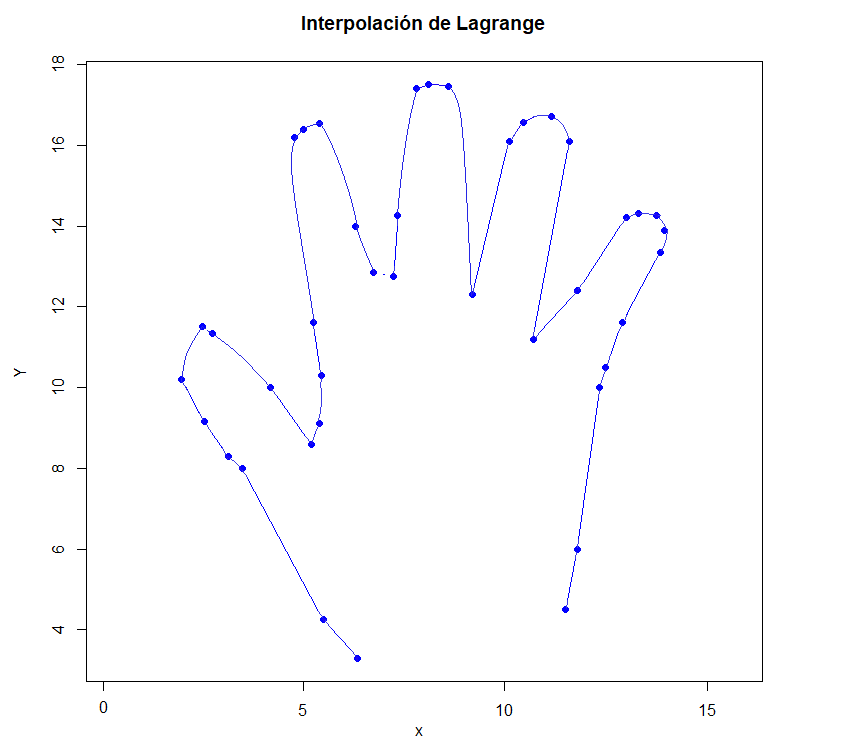
\includegraphics[scale=0.38]{img/1ra-InterpolaciónLagrange.PNG}
\vspace{-1em}
\caption{Primera interpolación de Lagrange}
\label{fig:lagrange-inicial}
\end{figure} 

En la figura \ref{fig:original-vs-lagrange}, se encuentra la comparación entre la trayectoria no interpolada de la hormiga, y la generada de interpolación mediante Lagrange.

\begin{figure}[ht!]
\centering
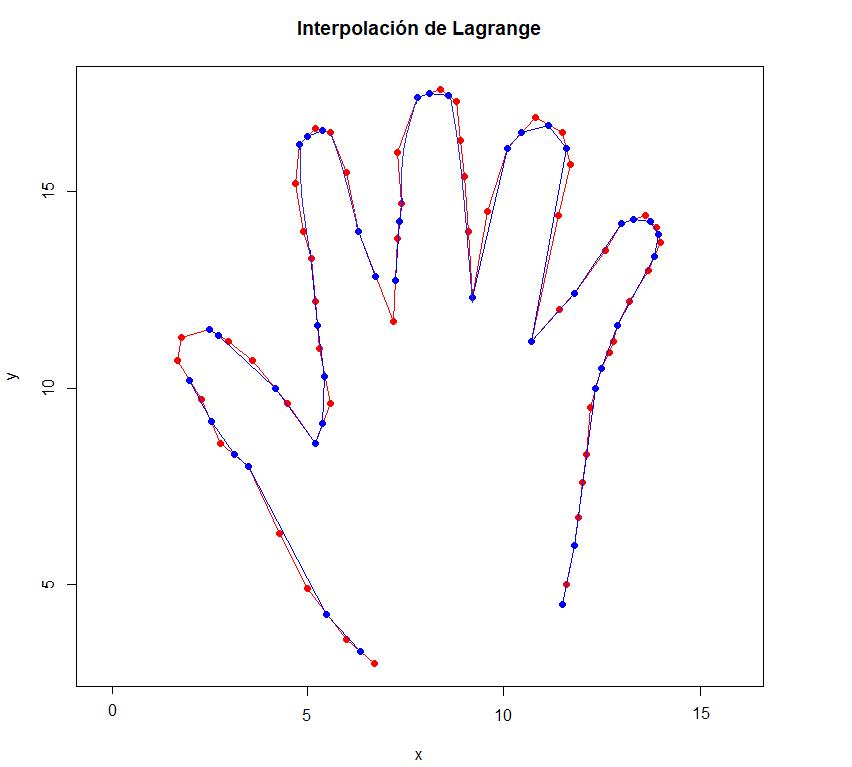
\includegraphics[scale=0.38]{img/Comparación Original-Lagrange.PNG}
\vspace{-1em}
\caption{Comparación entre trayectoria original y trayectoria generada por interpolación de Lagrange}
\label{fig:original-vs-lagrange}
\end{figure}

\subsection{Reconstrucción mediante Splines}

Para reconstruir la trayectoria de la hormiga, también se decidió utilizar la interpolación mediante Splines. La particularidad de esta solución, es que necesita la división del conjunto de puntos en varios subconjuntos de puntos, generando así, múltiples funciones interpolantes. \par

\subsubsection{Interpolación Inicial}

La reconstrucción inicial de la trayectoria, fue realizada tomando como base los $64$ puntos proporcionados por el problema, que fueron expuestos en la sección III. La realización de este proceso, requirió además el uso de 21 funciones interpolantes, que abarcaran todos los puntos.

En la figura \ref{fig:splines-inicial} se presenta la primera interpolación mediante Splines. \par

\begin{figure}[ht!]
\centering
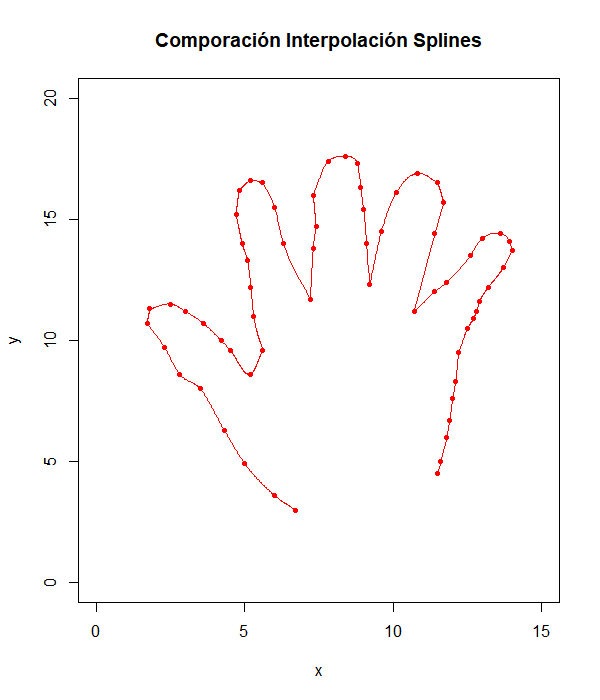
\includegraphics[scale=0.5]{img/splines_inicial.png}
\vspace{-1em}
\caption{Primera interpolación de Splines}
\label{fig:splines-inicial}
\end{figure}

\subsubsection{Reducción de Puntos}

Después de haber hecho una interpolación inicial de la mano, se encuentra que hay muchos puntos cuya información no es relevante para la obtención de la trayectoria. Es por esto que el siguiente paso que se tiene en cuenta, es la reducción de los puntos utilizados para obtener la solución. \par

En total, se pudo reducir la cantidad hasta $43$ puntos, y $20$ funciones interpolantes. A continuación se presentan los puntos obtenidos:

$x=($6.7, 5.0, 3.5, 2.8, 2.3, 1.7, 1.8, 2.5, 3.0, 4.5, 5.2, 5.6, 5.3, 5.1, 4.7, 4.8, 5.2, 5.6, 6.0, 6.3, 7.2, 7.4, 7.3, 7.8, 8.4, 8.8, 8.9, 9.2, 10.1, 10.8, 11.5, 11.7, 10.7, 12.6, 13.0, 13.6, 13.9, 14.0, 12.9, 12.8, 12.2, 12.0, 11.5$)$ \par

$x=($3.0, 4.9, 8.0, 8.6, 9.7 10.7 11.3 11.5 11.2, 9.6, 8.6, 9.6, 11.0, 13.3, 15.2, 16.2, 16.6, 16.5, 15.5, 14.0, 11.7, 14.7, 16.0, 17.4, 17.6, 17.3, 16.3, 12.3, 16.1, 16.9, 16.5, 15.7, 11.2, 13.5, 14.2, 14.4, 14.1, 13.7, 11.6, 11.2, 9.5, 7.6, 4.5$)$ \par

En la figura \ref{fig:splines-reducida} se presenta la interpolación reducida mediante Splines. \par

\begin{figure}[ht!]
\centering
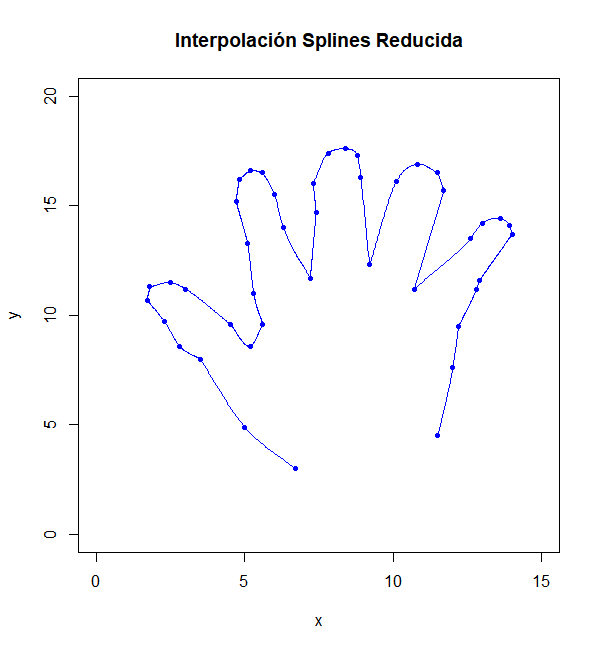
\includegraphics[scale=0.5]{img/splines_reducida.png}
\vspace{-1em}
\caption{Interpolación Splines de puntos reducidos}
\label{fig:splines-reducida}
\end{figure}

\subsubsection{Cálculo del Error}

Debido a que ocurrió una reducción del $32.81\%$ en la cantidad de puntos, es inevitable que haya alguna medida del error entre la primera interpolación de Splines, y la interpolación reducida. \par

El cálculo del error entre ambas interpolaciones fue realizada mediante la resta de ambas funciones interpolantes en el intervalo interpolado. \par

\[ E(x)=|f_1(x) - f_2(x)|\]

Se hizo un promedio de $E(x)$ para todo el intervalo, obteniendo como resultado un error promedio menor a $1.3*10^{-7}$. En la figura \ref{fig:comparacion-splines} se puede observar la comparación entre ambos resultados de las interpolaciones con Splines. \par

\begin{figure}[ht!]
\centering
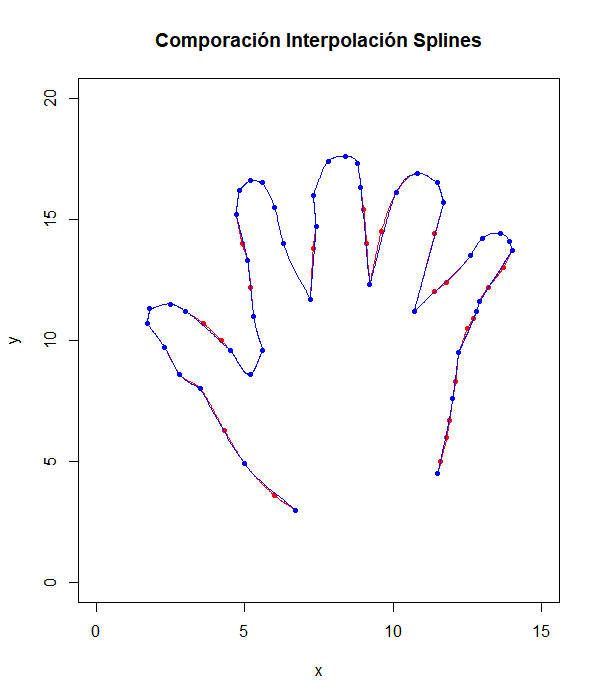
\includegraphics[scale=0.5]{img/comparacion_splines.png}
\vspace{-1em}
\caption{Comparación de la Interpolación Splines}
\label{fig:comparacion-splines}
\end{figure}

\section{Conclusiones}

Después de realizar toda la investigación e implementación de los algoritmos utilizando librerías internas y externas para calcular la interpolación de un conjunto de puntos mediante métodos numéricos, así como la optimización de puntos para reducir la información, podemos concluir que existen diferentes metodologías para resolver problemas de interpolación, y que es de suma importancia identificar cuales son las virtudes y defectos de los distintos métodos númericos que se pudieran aplicar. \par

Comparando los resultados obtenidos, se puede concluir que para el problema tratado, la interpolación mediante Splines es uno de los algoritmos más apropiados para dar una solución. Esta arrojó resultados de curvas más suevas y precisas a lo que pudiera ser la imagen inicial de donde fue extraída la información. \par

Adicionalmente, los conceptos abordados son de suma importancia, ya que pueden representar problemas de la vida cotidiana. Aunque el problema planteado no pareciera estar relacionado con dimensiones de la vida real, realmente representa una de la gran cantidad de aplicaciones que puede tener la interpolación en distintas disciplinas. En la meteorología, por ejemplo, puede ser utilizada para estimar las posibles mediciones climáticas que pudieran tenerse en un cuerpo geográfico (aunque esta dependa también de la extrapolación). \par

Cabe resaltar que distintos resultados serán propiciados, dependiendo de los métodos y algoritmos que sean implementados. Existen otros métodos de interpolación que no fueron abordados en este documento, y que pueden ser utilizados en otras aplicaciones. \par

\begin{thebibliography}{00}
\bibitem{b1} R. L. Burden y J. D. Faires, Numerical analysis, 9th ed. Boston, MA: Brooks/Cole, Cengage Learning, 2011.
\bibitem{b2} J. L. O’Connor, Ingeniería de los Algoritmos y Métodos Numéricos, 2.a ed. España: Círculo Rojo, 2017.
\end{thebibliography}

\end{document}
